%===================================================================================
% JORNADA CIENTÍFICA ESTUDIANTIL - MATCOM, UH
%===================================================================================
% Esta plantilla ha sido diseñada para ser usada en los artículos de la
% Jornada Científica Estudiantil, MatCom.
%
% Por favor, siga las instrucciones de esta plantilla y rellene en las secciones
% correspondientes.
%
% NOTA: Necesitará el archivo 'jcematcom.sty' en la misma carpeta donde esté este
%       archivo para poder utilizar esta plantila.
%===================================================================================



%===================================================================================
% PREÁMBULO
%-----------------------------------------------------------------------------------
\documentclass[a4paper,10pt,twocolumn]{report}

%===================================================================================
% Paquetes
%-----------------------------------------------------------------------------------
\usepackage{amsmath}
\usepackage{amsfonts}
\usepackage{amssymb}
\usepackage{jcematcom}
\usepackage[utf8]{inputenc}
\usepackage{listings}
\usepackage[pdftex]{hyperref}
\usepackage{float}
\usepackage{graphicx}
\usepackage{listings}
%-----------------------------------------------------------------------------------
% Configuración
%-----------------------------------------------------------------------------------
\hypersetup{colorlinks,%
	    citecolor=black,%
	    filecolor=black,%
	    linkcolor=black,%
	    urlcolor=blue}

\lstset{ %
	language=R, % lenguaje
	basicstyle=\footnotesize\ttfamily,
	tabsize=2,
	stringstyle=\ttfamily,
	keywordstyle=\color{blue},
	commentstyle=\color{brown}
	showstringspaces=false
}
			
%===================================================================================



%===================================================================================
% Presentacion
%-----------------------------------------------------------------------------------
% Título
%-----------------------------------------------------------------------------------
\title{Proyecto de Estadística Segunda Fase - Household}

%-----------------------------------------------------------------------------------
% Autores
%-----------------------------------------------------------------------------------
\author{\\
\name Loraine Monteagudo García \email \href{mailto:l.monteagudo@estudiantes.matcom.uh.cu}{l.monteagudo@estudiantes.matcom.uh.cu}
	\\ \addr Grupo C411 \AND
\name Amanda Marrero Santos \email \href{mailto:a.marrero@estudiantes.matcom.uh.cu}{a.marrero@estudiantes.matcom.uh.cu}
  \\ \addr Grupo C411 \AND
  \name Manuel S. Fernández Arias \email \href{mailto:m.fernandez2@estudiantes.matcom.uh.cu}{m.fernandez2@estudiantes.matcom.uh.cu}
	\\ \addr Grupo C411}

%-----------------------------------------------------------------------------------
% Tutores
%-----------------------------------------------------------------------------------
\tutors{\\
Msc. Dalia Díaz Sistach, \emph{Universidad de la Habana, Facultad de Matemática y Computación}}

%-----------------------------------------------------------------------------------
% Headings
%-----------------------------------------------------------------------------------
\jcematcomheading{\the\year}{1-\pageref{end}}{Loraine Monteagudo, Amanda Marrero, Manuel Fernández}

%-----------------------------------------------------------------------------------
\ShortHeadings{Household}{Autores}
%===================================================================================



%===================================================================================
% DOCUMENTO
%-----------------------------------------------------------------------------------
\begin{document}

%-----------------------------------------------------------------------------------
% NO BORRAR ESTA LINEA!
%-----------------------------------------------------------------------------------
\twocolumn[
%-----------------------------------------------------------------------------------

\maketitle

%===================================================================================
% Resumen y Abstract
%-----------------------------------------------------------------------------------
\selectlanguage{spanish} % Para producir el documento en Español

%-----------------------------------------------------------------------------------
% Resumen en Español
%-----------------------------------------------------------------------------------
% \begin{abstract}

% 	El Resumen en Español debe constar de $100$ a $200$ palabras y presentar de forma
% 	clara y concisa el contenido fundamental del artículo.

% \end{abstract}

%-----------------------------------------------------------------------------------
% English Abstract
%-----------------------------------------------------------------------------------
\vspace{0.5cm}

% \begin{enabstract}

%   The English Abstract must have have $100$ to $200$ words, and present in a clear
%   and concise form the essentials of the article content.

% \end{enabstract}

%-----------------------------------------------------------------------------------
% Palabras clave
%-----------------------------------------------------------------------------------
% \begin{keywords}
% 	Separadas,
% 	Por,
% 	Comas.
% \end{keywords}

%-----------------------------------------------------------------------------------
% Temas
%-----------------------------------------------------------------------------------
% \begin{topics}
% 	Tema, Subtema.
% \end{topics}


%-----------------------------------------------------------------------------------
% NO BORRAR ESTAS LINEAS!
%-----------------------------------------------------------------------------------
\vspace{0.8cm}
]
%-----------------------------------------------------------------------------------


%===================================================================================

%===================================================================================
% Introducción
%-----------------------------------------------------------------------------------
\section{Introducción}\label{sec:intro}
%-----------------------------------------------------------------------------------
 
 El estudio de la estadística es de vital importancia para el desarrollo de la sociedad moderna. Este proyecto usa los datos de UCI Machine Learning Repository, en particular el data set "Individual Household Electric Power Consumption". Se analiza un ejemplo real relacionado con el consumo eléctrico de una casa durante 4 años. Nuestro objetivo será realizar un estudio de estos datos usando técnicas de regresión, lo que nos permitirá determinar si existen relaciones lineales entre algunas de las variables dadas. Luego reduciremos la dimensión de los datos mediante el análisis de componentes principales (ACP), clusters y árboles de clasificación, haciendo además una interpretación de los mismos. Por último realizaremos un análisis de varianza o ANOVA para comparar las medias de una característica en varias poblaciones.

%===================================================================================

%-----------------------------------------------------------------------------------
	\subsection{Datos}\label{sub:datos}
%-----------------------------------------------------------------------------------
	El conjunto de datos contiene 2075259 mediciones del consumo eléctrico recolectadas en una casa entre diciembre de 2006 y noviembre de 2010 (47 meses).
	
	El data set contiene 9 variables que son:
	\begin{itemize}
		\item \textit{date}: La fecha en el formato dd/mm/yy
		\item \textit{time}: El tiempo en el formato hh:mm:ss
		\item \textit{global\_active\_power}: la corriente global activa de una casa promediada por minuto (en kilowatt). La corriente activa global es la potencia consumida por dispositivos distintos de los dispositivos asignados a los submedidores. La potencia activa global es el consumo de energía real, es decir, la consumida por aparatos eléctricos distintos de los aparatos submedidos.
		\item \textit{global\_reactive\_power}: la corriente global reactiva de una casa promediada por minuto (en kilowatt). La corriente reactiva global es la potencia que rebota y hace espuma sin ningún uso o fuga. Es el consumo de energía imaginario.
		\item \textit{voltage}: el voltaje promediado por minuto (en volt)
		\item \textit{global\_intensity}: la intensidad promediada por minuto de toda la casa (en kilowatt). Es la magnitud de la energía consumida. También llamada como fuerza de la corriente.
		\item \textit{sub\_metering\_1} (submedida1): Le corresponde a la cocina, conteniendo el lavavajillas, un horno y un microwave (en watt-hora de energía activa)
		\item \textit{sub\_metering\_2} (submedida2): Le corresponde al cuarto de lavado, conteniendo la lavadora, una secadora, un refrigerador y una luz (en watt-hora de energía activa)
		\item \textit{sub\_metering\_3} (submedida3: Le corresponde a un calentador de agua eléctrico y un aire acondicionado (en watt-hora de energía activa)
	\end{itemize}
	
	Como se puede apreciar, el data set tiene el inconveniente de que las variables están en medidas diferentes, lo que dificulta su comparación. Además, presenta valores perdidos, lo que ocasionó que se tuvieran que eliminar varias filas. Aún así, se tienen gran cantidad de datos con 2049280 observaciones reales, lo que dificultó su procesamiento y su análisis. Por ejemplo, varios diagramas de dispersión  y boxplots mostraron muy poca información al tener tantos puntos para representar. 
	
%===================================================================================
% Desarrollo
%-----------------------------------------------------------------------------------
%-----------------------------------------------------------------------------------
\section{Técnicas de Regresión}\label{sub:regression}
%-----------------------------------------------------------------------------------
	
	La idea detrás de la regresión lineal simple es encontrar el modelo lineal que mejor se ajusta a los datos. Para decidir si nuestros datos se ajustan al modelo de Regresión Lineal Simple es necesario que se cumpla una serie de suposiciones a las que se les llama supuestos del modelo. Este modelo puede ser expresado como: $Y=X\beta + \epsilon$
	
	Para elegir las variables con las que realizaremos la regresión primero veamos su relación mediante la matriz de correlación mostrada de manera simplificada en la Figura \ref{fig:cor_matrix}
	
	
	\begin{figure}[htb]
		\centering
		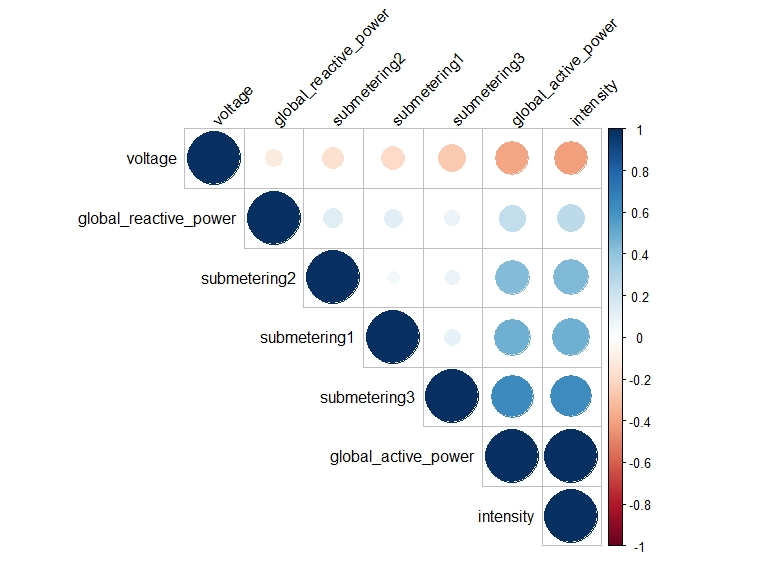
\includegraphics[width=\linewidth]{img/regression/cor_matrix}
		\caption{Forma gráfica de la matriz de correlación}
		\label{fig:cor_matrix}
	\end{figure}
	
	Se observa una relación lineal entre la Corriente Global Activa y la Intensidad, siendo su coeficiente de correlación cercano a 1. Esta suposición se respalda por el diagrama de dispersión de la Intensidad y la Corriente Global Activa mostrada en la Figura \ref{fig:intensity_gap}.
	
	\begin{figure}[h]
	\centering
	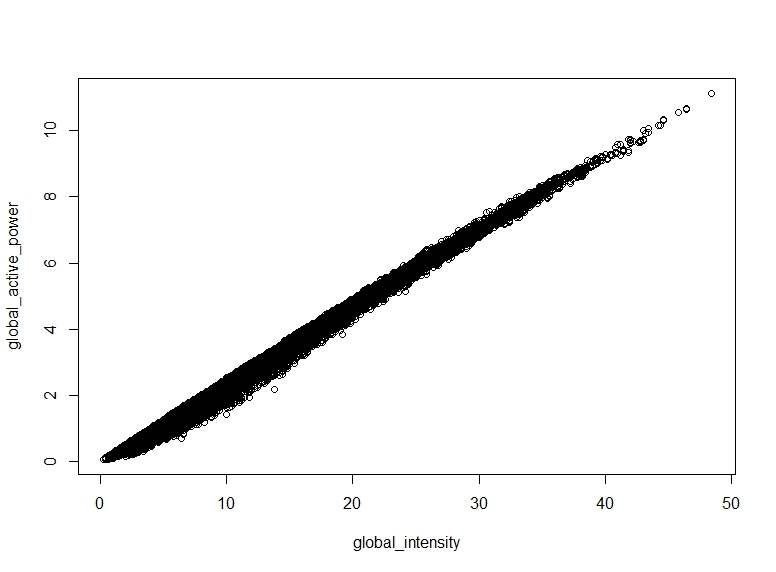
\includegraphics[width=\linewidth]{img/regression/intensity_gap}
	\caption{Diagrama de dispersión de la intensidad y la corriente global activa}
	\label{fig:intensity_gap}
	\end{figure}

	Por lo tanto, se decide realizar la regresión lineal entre la Intensidad y la Corriente Global Activa. El resultado al ejecutar dicha regresión fue el siguiente:
	
	\begin{figure}[H]
		\centering
		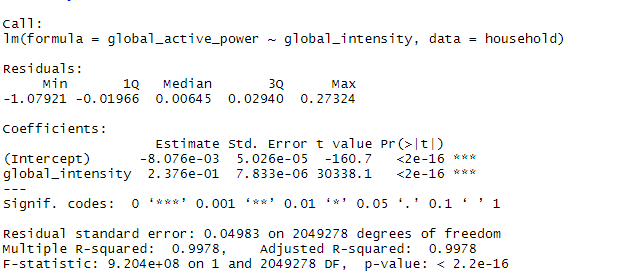
\includegraphics[width=1\linewidth]{img/regression/lm}
		\caption{Salida del Modelo de Regresión múltiple}
		\label{fig:lm}
	\end{figure}
	
	Los valores de $\beta_0$ y $\beta_1$ se obtienen de la columna de estimados. El modelo con los coeficientes sustituidos sería:
	
	\begin{equation*}
		gap = -8.07e^{-3} + 0.237*global\_intensity
	\end{equation*}
	
	Análisis del \textit{summary}:
	\begin{itemize}
		\item \textit{Residuals}: Es el error entre la predicción del modelo y los resultados reales. Se observan valores relativamente pequeños, lo que contribuye a la robustez del modelo.
		\item \textit{Coefficients}: 
		\begin{itemize}
			\item \textit{Std Error}: tiene valores bajos, lo que parece indicar una buena precisión del estimador
			\item \textit{t-value} y $Pr(>t)$: Como $Pr(>t)$ es menor que 0.05 entonces la prueba es significativa   
		\end{itemize}
		\item \textit{Performance Measures}
		\begin{itemize}
			\item \textit{Residual Standard Error}: Se obtienen pequeños valores
			\item \textit{Multiple / Adjusted R-Square}: Estos valores son bastantes cercanos a 1, por lo que el modelo explica bastante la variación.
			\item \textit{F-Statistic}: El valor del estadígrafo F es menor que 0.05 así que podemos afirmar que existe al menos una variable significativamente diferente a cero en el modelo.
		\end{itemize}
	\end{itemize}
	
	A la hora de analizar los residuos para comprobar que se cumplen los supuestos del modelo tenemos que analizar cuatro cuestiones con respecto a los residuos:
	
	\begin{enumerate}
		\item La media y la suma de los errores es cero.
		
		Como se puede observar en el siguiente código este supuesto se cumple:
		\begin{lstlisting}
		> mean(model$residuals)
		-8.040966e-16
		> sum(model$residuals)
		-1.643985e-09
		\end{lstlisting}
		\item Errores normalmente distribuidos.	
		
		\begin{figure}[H]
			\centering
			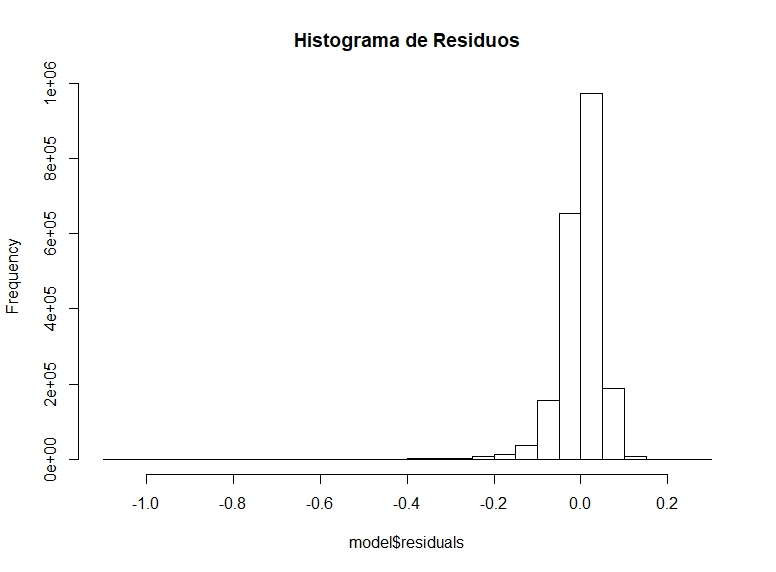
\includegraphics[width=0.9\linewidth]{img/regression/histogram}
			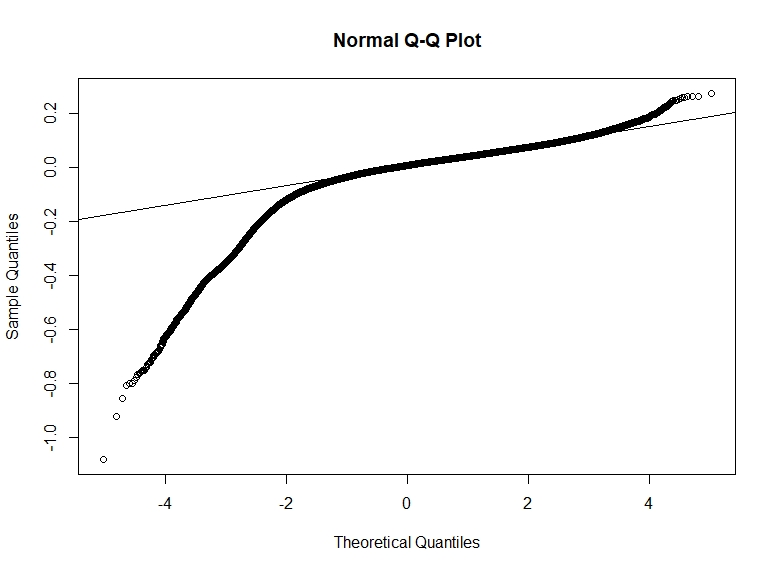
\includegraphics[width=0.9\linewidth]{img/regression/normal_qq_plot}
			\label{fig:histogram}
			\caption{Salida de los residuos del modelo de Regresión Múltiple}
		\end{figure}
		
		El histograma de residuos y el QQ-plot mostrados en la Figura \ref{fig:histogram} son formas de evaluar visualmente si los residuos siguen una distribución normal. El histograma se asemeja a la distribución normal siguiendo el patrón de campana, sin embargo, el QQ-plot muestra bastante desviación con respecto a la línea normal, por lo tanto, para asumir la normalidad de los errores nos apoyamos en el test de Shapiro-Wilk:
		
		\begin{figure}[H]
			\centering
			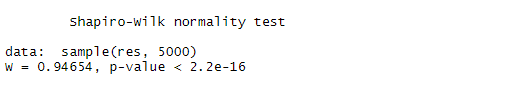
\includegraphics[width=\linewidth]{img/regression/shapiro-wilk}
			\caption{Prueba de normalidad de Shapiro-Wilk}
			\label{fig:shapiro-wilk}
		\end{figure}
		Se tomó una muestra de 5000 residuos ya que es la cantidad máxima de valores que puede recibir este test. Como $p-value = 2.2e^{16} < 0.05$ entonces no se puede rechazar la hipótesis nula, por lo que los errores no siguen una distribución normal.
		
		Solo por un propósito ilustrativo continuaremos analizando los supuestos pero ya al incumplirse el de normalidad podemos concluir que el modelo no es válido.
		
		\item Independencia de los residuos
		
		La prueba Durbin-Watson se utiliza para verificar si los residuos son independientes. La hipótesis nula de esta prueba es que los errores son independientes.
		
		\begin{figure}[H]
			\centering
			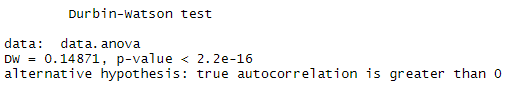
\includegraphics[width=\linewidth]{img/regression/durbin-watson}
			\caption{Prueba para la independencia de los residuos de Dubin-Watson}
			\label{fig:durbin-watson}
		\end{figure}
		
		Como se observa en la Figura \ref{fig:durbin-watson} el $p-valor$ de esta prueba es menor que $2.2e-16 < 0.05$ entonces podemos rechazar la hipótesis nula, por lo que los errores no son independientes, incumpliéndose el supuesto de independencia.
		
		\item La varianza de los errores es constante (Homocedasticidad)
		
		\begin{figure}[H]
			\centering
			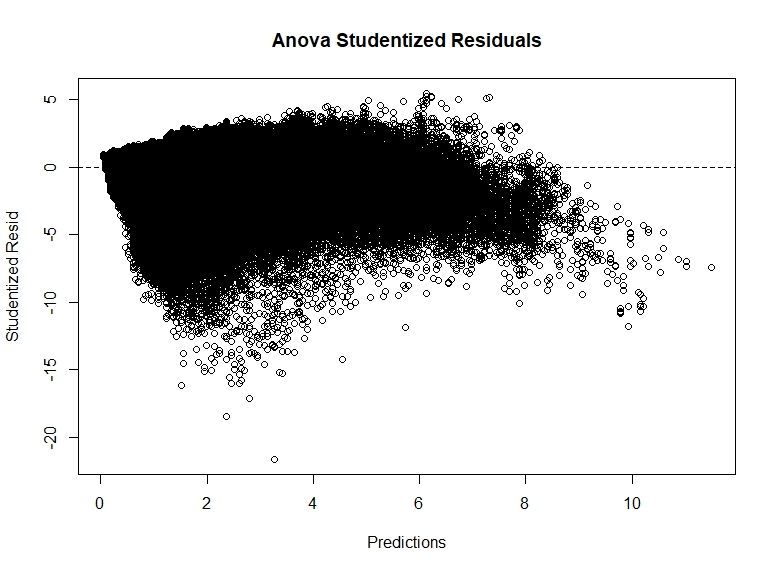
\includegraphics[width=0.7\linewidth]{img/regression/studentized}
			\caption{Gráfico estandarizado de los residuos}
			\label{fig:studentized}
		\end{figure}
		
		Por el gráfico de los residuos estandarizados mostrado en la Figura \ref{fig:studentized} no parece que el supuesto de Homocedasticidad se cumpla.	
		
		Lo comprobamos con la prueba de Breusch-Pagan:
		
		\begin{figure}[H]
			\centering
			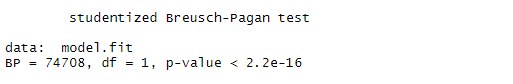
\includegraphics[width=\linewidth]{img/regression/studentized_test}
			\caption{Gráfico estandarizado de los residuos}
			\label{fig:studentized_test}
		\end{figure}
		
		Como el $p-valor = 2.2e-16 < 0.05$ se puede rechazar la hipótesis nula, por lo tanto no se cumple la Homocedasticidad tampoco.
		
	\end{enumerate}
		
	Con el objetivo de encontrar un modelo de regresión lineal que cumpliese los supuestos se probaron distintas combinaciones de variables adicionales aplicando regresión múltiple. Además, se intentó excluir registros con el objetivo de disminuir el tamaño de la muestra. Sin embargo, no se encontró una combinación que cumpliese con dichos supuestos.
		
%-----------------------------------------------------------------------------------
	\section{Reducción de dimensión}\label{sub:acp}
%-----------------------------------------------------------------------------------
	\subsection{Análisis de Componentes Principales (ACP)}

	Una de las formas de realizar la reducción de la dimensión es a través del análisis de componentes principales (ACP). Se busca obtener de las n variables de un sistema un subconjunto de tamaño k, las cuales provean tanta información como las n variables originales. Este análisis tiene el objetivo de revelar relaciones entre variables de las que no se tenía sospecha, permitiendo interpretaciones que realizando un análisis ordinario quizá no encontraríamos. Por ejemplo, podemos obtener mediante este estudio variables incorrelacionadas entre sí.
	
	En nuestro data set hay un total de 9 variables, el análisis de los componentes principales se realiza con las variables que tienen un valor numérico, por lo que excluimos la fecha y la hora. Por lo tanto analizamos: la corriente global activa, la corriente global reactiva, el voltaje, la intensidad global y otras mediciones secundarias como el consumo activo de energía en watt-hora de la cocina (submedida1), el cuarto de lavado (submedida2) y el correspondiente a un calentador de agua y un aire acondicionado (submedida3). 
	
	Para determinar la relación entre las variables tenemos que calcular la matriz de correlación que se muestra en la Figura \ref{fig:corr_matrix}.
	
	\begin{figure*}[hbt]
	\centering
	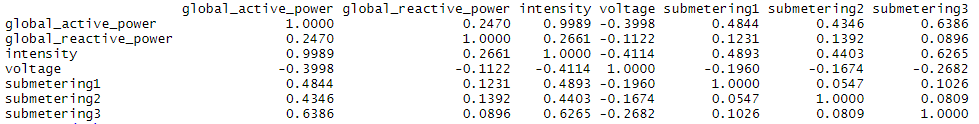
\includegraphics[width=2\columnwidth]{img/acp/corr_matrix}
	\caption{Matriz de correlación}  
	\label{fig:corr_matrix}
	\end{figure*}
	
	Por desgracia esta matriz es muy grande por lo que resulta fácil perdernos, para un mejor análisis se usa la función \texttt{symnum} obteniendo:
	
	\begin{table}[H]
		\scalebox{0.85}{
		\begin{tabular}{lccccccc}
			                   & GAP & GRP & I & V & S1 & S2 & S3 \\
			Corriente Activa   &  1  &     &   &   &    &    &  \\
			Corriente Reactiva &     &  1  &   &   &    &    &  \\
			Intensidad         &  B  &     & 1 &   &    &    &  \\
			Voltaje            &  .  &     & . & 1 &    &    &  \\
			Submedida1         &  .  &     & . &   & 1  &    &  \\
			Submedida2         &  .  &     & . &   &    & 1  &  \\
			Submedida3         &  ,  &     & , &   &    &    & 1
		\end{tabular}}
		[1] 0 ‘ ’ 0.3 ‘.’ 0.6 ‘,’ 0.8 ‘+’ 0.9 ‘*’ 0.95 ‘B’ 1
		\label{tab:syn_matrix}
		\caption{Matriz de correlación usando \texttt{symnum}}
	\end{table}
	
	Como se puede observar en el Cuadro 1 y en la Figura \ref{fig:cor_matrix} no es altamente correlacionada la matriz, exceptuando por algunas variables como la intensidad y la corriente global activa que están altamente relacionadas.
	
	\subsubsection{Importancia de los componentes:}
	
	
	\begin{figure}[h]
	\centering
	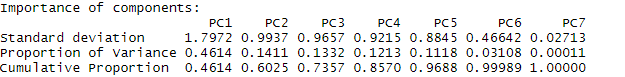
\includegraphics[width=\linewidth]{img/acp/importance}
	\caption{Importancia de los componentes}
	\label{fig:importance}
	\end{figure}
	
	Se puede observar en la Figura \ref{fig:importance} que con las 4 primeras componentes podemos explicar el 85\% de la muestra, sin embargo, es suficiente con una proporción acumulativa  superior al 70\%, por lo que solo nos quedaríamos con las tres primeras. Según el criterio Kaiser elegiríamos las componentes q tengan valor propio $\lambda_m$ mayor que 1, sin embargo, esto solo lo cumple la primera componente, pero se puede tomar un punto de corte $\lambda^* = 0.7$ en cuyo caso se cumpliría para las 5 primeras. De acuerdo al análisis realizado y al gráfico de la Figura \ref{fig:1} nos quedamos con las 3 primeras ya que no se aprecia que haya mucha variabilidad en las componentes restantes.
	
	\begin{figure}[H]
		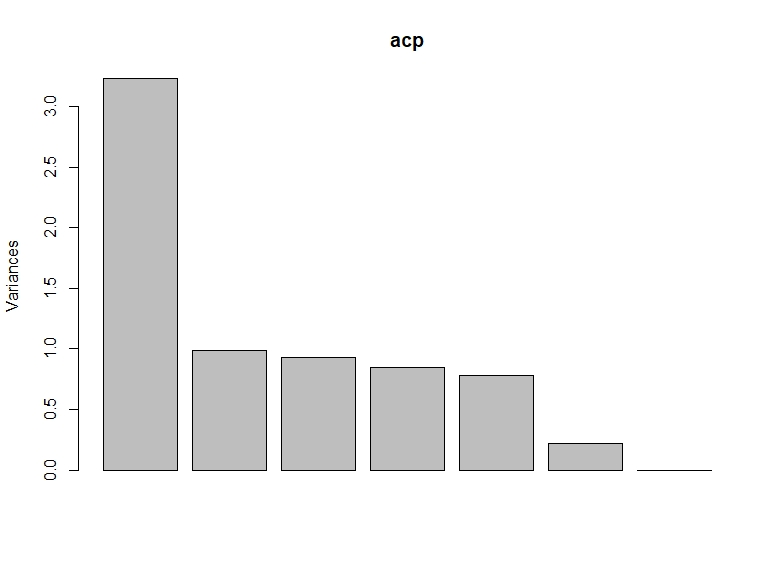
\includegraphics[width=0.9\linewidth]{img/acp/acp.jpeg}
		\caption{Gráfico de las Componentes Principales}
		\label{fig:1}
	\end{figure}
	
	Ahora analizamos la matriz de valores propios y así sabremos qué variables son importantes para cada componente y en qué medida.
	
	\begin{table}[ht]
	\begin{tabular}{lccc}
		                   &   PC1   &   PC2   &   PC3   \\
		Corriente Activa   & -0.5381 & 0.0511  & 0.0298  \\
		Corriente Reactiva & -0.1868 & -0.6704 & -0.3403 \\
		Intensidad         & -0.5398 & 0.0317  & 0.0191  \\
		Voltaje            & 0.2961  & -0.1424 & -0.0595 \\
		Submedida1         & -0.2953 & 0.1005  & -0.7409 \\
		Submedida2         & -0.2661 & -0.5733 & 0.5005  \\
		Submedida3         & -0.3721 & 0.4336  & 0.2828
	\end{tabular}
	\label{tab:3}
	\caption{Matriz de valores propios}
	\end{table}
	
	Comencemos por la primera componente, tomamos el mayor valor propio modular 0.2953 y lo dividimos entre 2, esto da 0.148 todo valor propio cuyo modulo esté por encima de 0.148 en la columna de PC1 nos dará las variables que conforman esta componente. Por tanto, la interpretación sería que la PC1 está caracterizada por un impacto negativo de todas las variables involucradas. Lo que quiere decir que es una muestra con baja corriente global activa, baja corriente global reactiva, baja intensidad y la corriente consumida en las submediciones 1, 2 y 3 son bajas también.
	
	Siguiendo el mismo análisis con la segunda componente el máximo valor propio es 0.4336, por lo que existe una baja corriente global reactiva y un bajo consumo de energía en la submedición 2 correspondiente al cuarto de lavado.

	La tercera componente nos muestra un alto consumo en la submedida 3 correspondiente al calentador de agua eléctrico y el aire acondicionado y bajos valores de corriente global reactiva y en la submedida 1 correspondiente a la cocina.
	
	\subsection{Clusters}
	
	Otra técnica popular de reducción de dimensiones es el clúster. La idea básica del clúster es clasificar objetos formando grupos que sean lo más homogéneos posibles dentro de sí mismos y heterogéneos entre sí. Por tanto, el número de clusters dependen de lo que consideremos como similar. El análisis de clúster es una tarea de clasificación que puede ser vista desde dos puntos de vistas diferentes:
	\begin{enumerate}
		\item Clúster por particiones: se usan cuando conocemos cuántos grupos hay. Producen una partición de los objetos en un número especificado de grupos siguiendo un criterio de optimización. El algoritmo usado para generar este tipo de clusters es el de \textit{K-Means}
		\item Clúster Jerárquico: se usan cuando no conocemos cuántos grupos hay. Producen una secuencia de particiones, juntando o separando clusters. En cada paso se juntan o separan dos clusters siguiendo algún criterio especificado.
	\end{enumerate}
	
	Para realizar el análisis de los datos por clúster al igual que con ACP, se eligieron las variables que tienen un valor numérico, excluyendo la fecha y la hora.
	
	Antes de elegir el tipo de clúster vamos a estandarizar los datos para evitar errores en la clasificación por cuestiones de variabilidad en las unidades de medida. Para esto usaremos la fórmula:
	
	\begin{equation*}
		Z_i = \dfrac{X_i - \mu_i}{\sigma_i}
	\end{equation*}
	
	Como se puede observar en la Figura \ref{fig:dispersion_cluster}, los datos estandarizados tienen el mismo comportamiento que los que no fueron estandarizados, la diferencia está en la escala de las mediciones que es similar. Trabajaremos con las mediciones escaladas.
	
	\begin{figure}[H]
	\centering
	\includegraphics[width=0.9\linewidth]{"img/cluster/diagrama de dispersion estandarizado"}
	\includegraphics[width=0.9\linewidth]{"img/cluster/diagrama de dispersion"}
	\caption{Diagrama de dispersión de los datos estandarizados y sin estandarizar tomando como ejemplo la corriente global activa y la corriente global reactiva}
	\label{fig:dispersion_cluster}
	\end{figure}
	 	
	 \subsubsection{Clusters Jerárquicos}
	 A continuación nos dispusimos a realizar el clúster jerárquico, sin embargo debido a la gran cantidad de datos fue imposible procesar una matriz de distancia tan grande. A pesar de esto, con el objetivo de encontrar un k adecuado para el algoritmo de k-means se realizó el clúster jerárquico con una muestra de los registros. Distintas formas de obtener una muestra fueron probadas (cogiendo los registros de un día determinado, filas al azar) y distintos tamaños, ninguno de los cuales dio una diferencia significativa en la cantidad de dendograma del clúster jerárquico. Este se muestra en la Figura \ref{fig:dendogram} a pesar de que no es posible analizarlo adecuadamente por la gran cantidad de datos:
	 
	\begin{figure}[H]
	\centering
	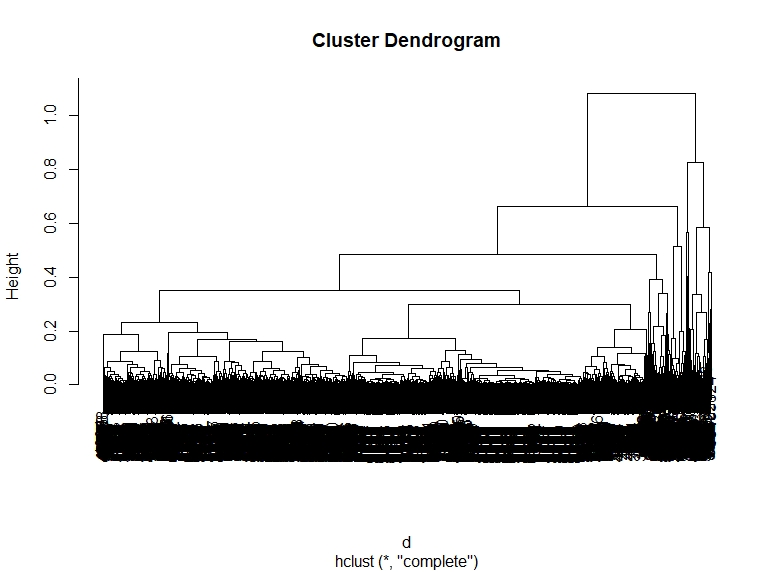
\includegraphics[width=0.9\linewidth]{img/cluster/dendogram}
	\caption{Dendograma de Clúster Jerárquico. Ajuste Completo}
	\label{fig:dendogram}
	\end{figure}
	
	Tomando como altura 0.4 tenemos 8 clusters, por lo que ese es el k que utilizaremos en el algoritmo de K-Means.
	
	\subsubsection{K-means}
	
	Habiendo realizado la clasificación por el método jerárquico comenzamos eligiendo el k a partir del número de clusters encontrado previamente. Por lo tanto, comenzamos con k=8. Se realizó el experimento con distintos valores de k, sin embargo, con este número fue como se obtuvieron mejores resultados, teniendo una similitud de 87.5\% entre los elementos de cada clúster como se puede apreciar en la Figura \ref{fig:k-means}
		
	\begin{figure*}[ht]
	\centering
	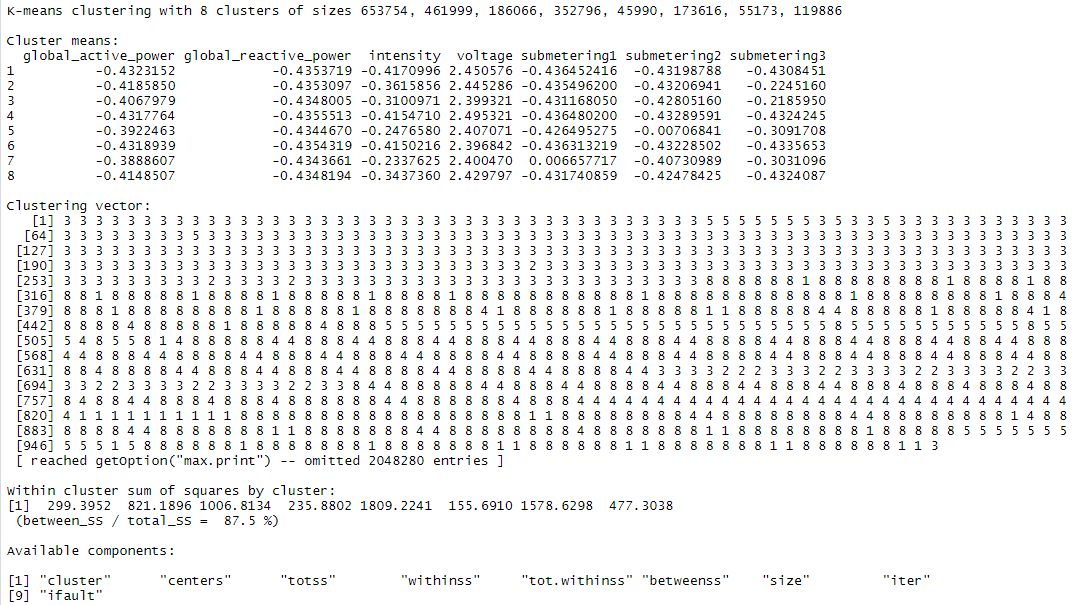
\includegraphics[width=1.8\columnwidth]{img/cluster/k-means}
	\caption{Salida del algoritmo de K-means con 8 clusters}
	\label{fig:k-means}
	\end{figure*}
	
	Por la gran cantidad de datos no se puede analizar correctamente en un gráfico el resultado de k-means, por lo que para analizar las relaciones de forma visual entre variables debemos hacerlo de dos a dos, por ejemplo, en la Figura \ref{fig:clusters_gap_grp} se muestran los 8 clusters de la corriente global activa y la corriente global reactiva.
	
	\begin{figure}[H]
		\centering
		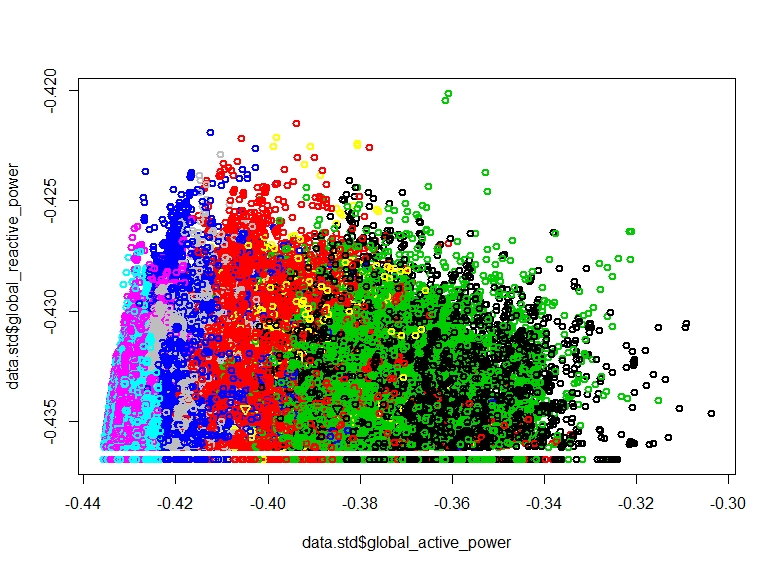
\includegraphics[width=0.9\linewidth]{img/cluster/clusters_gap_grp}
		\caption{K-Means con 8 graficando los clusters de la Corriente Global Activa y la Corriente Global Reactiva}
		\label{fig:clusters_gap_grp}
	\end{figure}

	\subsection{Árboles de Decisión }
	
	Los métodos basados en árboles de clasificación son poderosas herramientas analíticas para explorar estructuras de datos complejas, y una buena opción si necesitamos generar reglas que puedan entenderse y explicarse fácilmente. Su importancia viene dada porque nos permite encontrar variables claves que identifican los miembros de los grupos actuales, formular reglas para hacer predicciones sobre los miembros de grupos potenciales de nuevos casos y permiten desplegar gráfica y estadísticamente los resultados de los análisis, proporcionando una medida de confianza para ver cuán correcta es la clasificación.
	
	Uno de las mayores dificultades para realizar este análisis fue elegir qué variable intentar predecir ya que todas las variables del data set tienen un valor fraccionario que no los hacen adecuados para una técnica de clasificación, más bien es un problema de regresión. Así que tomamos la decisión de introducir una nueva variable que sería booleana para comprobar si una variable cumple una determinada propiedad. Vimos en la matriz de correlación al analizar los componentes principales (Cuadro \ref{tab:syn_matrix}) que esta no es altamente correlacionada, excepto por la intensidad y la corriente global activa, que están bastante relacionadas, por lo que consideramos interesante clasificar una de estas variables. Luego, con los datos numéricos del data set nos propusimos clasificar cuando la corriente global sobrepasa a su media.
	
	Al escoger los conjuntos de entrenamiento y de prueba se tomaron cuatro quintos de la población para entrenar y el quinto restante servirá para probar el árbol y calcular el error de clasificación. Como contamos con un data set grande, la quinta parte de este es lo suficientemente amplio para que los resultados obtenidos en el conjunto de prueba sean estadísticamente válidos.
	
	El árbol que se obtuvo al aplicar el algoritmo clasificando la corriente global activa que sobrepasa una determinada cantidad se muestra en la Figura \ref{fig:gap_tree}
	
	\begin{figure}[H]
	\centering
	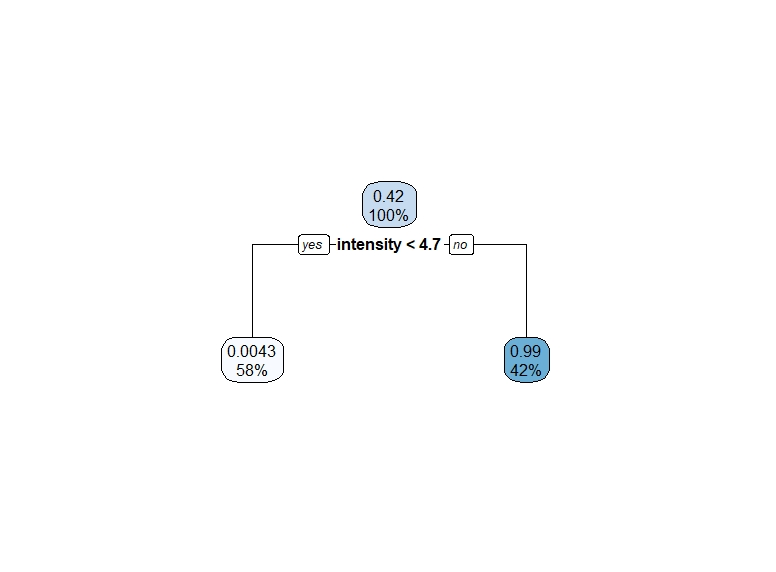
\includegraphics[width=\linewidth]{img/tree/gap_tree}
	\caption{Predicción de valores superiores a la media de la corriente global activa}
	\label{fig:gap_tree}
	\end{figure}
	
	Como se puede observar solo se necesita de la intensidad para predecir altos valores de la corriente global activa, lo que corrobora la alta relación entre estas dos variables. Se obtiene solo un error de 0.0045, lo que constituyen muy buenos resultados.
	
	Se probó hacer el mismo análisis con otra variable. Comprobamos si era posible predecir cuando estos valores excedían la media a partir de las otras variables. La más altamente relacionada después de la corriente global activa y la intensidad es la submedida3 (Tabla \ref{tab:syn_matrix}), y se obtuvo el árbol mostrado en la Figura \ref{fig:submetering3_tree}
	
	\begin{figure}[H]
		\centering
		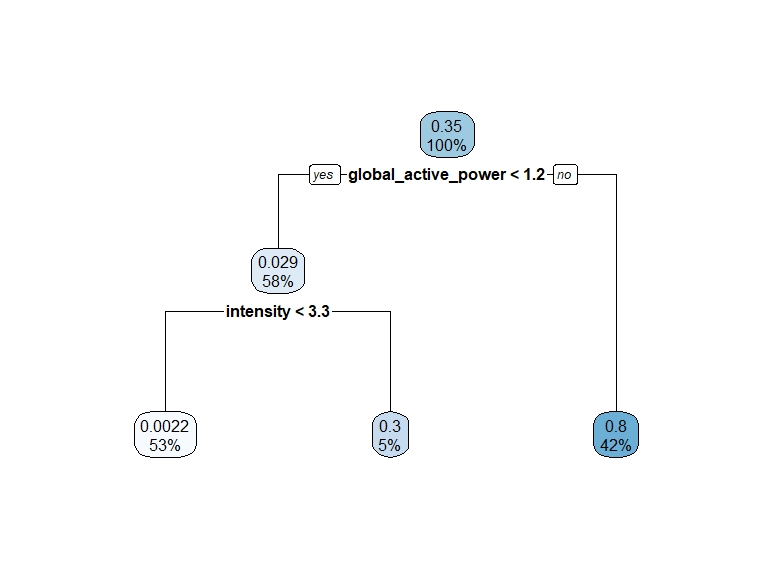
\includegraphics[width=\linewidth]{img/tree/submetering3_tree}
		\caption{Predicción de valores superiores a la media de la submedida3}
		\label{fig:submetering3_tree}
	\end{figure}
	
	De igual manera solo se necesitaron de dos variables para la predicción de la submedida3: la corriente global activa y la intensidad. Sin embargo, se obtuvo un error de 0.45, lo que representa un valor bastante alto.
	
%-----------------------------------------------------------------------------------
	\section{ANOVA}\label{sub:anova}
%-----------------------------------------------------------------------------------
	
	El análisis de varianzas o ANOVA a pesar de su nombre, es una técnica estadística que permite la comparación de las medias de una característica de varias poblaciones. Los ANOVA evalúan la importancia de uno o más factores al comparar las medias de la variable de respuesta en los diferentes niveles de los factores. Hacen una prueba de hipótesis para evaluar la similitud de las medias de dos o más poblaciones. La hipótesis nula establece que todas las medias de la población (medias de los niveles de los factores) son iguales mientras que la hipótesis alternativa establece que al menos una es diferente.
	
	Con el objetivo de cumplir los supuestos necesarios para que el experimento de ANOVA sea válido se utilizaron varios subconjuntos de variables. La relación entre la intensidad y la corriente global activa que fue ampliamente analizada en este trabajo fue una de las combinaciones que se probaron. Al igual que con la regresión lineal no se encontró combinación de variables que cumpliera los supuestos. Al final se decidió elegir la submedida3 (la variable que le corresponde al consumo de un calentador eléctrico y un aire acondicionado) como factor de interés y la corriente global activa y la intensidad como factores de bloque para analizar con mayor profundidad la relación existente entre estas variables. 
	
	Al elegir la intensidad y la corriente global activa como factores de bloque y la submedida3 como factor de interés no proponemos responder la interrogante ¿existen diferencias entre la submedida3 para los distintos valores de la corriente global activa y la intensidad?
	
	\begin{table}[H]
		\scalebox{0.7}{
		\begin{tabular}{lrrrrr}
			                 &      Df &   Sum Sq &  Mean Sq & F value &     $Pr(>F)$ \\
			Corriente Activa &       1 & 59482639 & 59482639 & 1562629 & $<2e-16$ *** \\
			Intensidad       &       1 &  8389201 &  8389201 &  220387 & $<2e-16$ *** \\
			Residuals        & 2049277 & 78007245 &       38 &         &  \\
			---              &
		\end{tabular}}
	   Signif. codes:  0 '***' 0.001 '**' 0.01 '*' 0.05 '.' 0.1 ' ' 1	  
	   \caption{Salida de anova con dos factores de bloque} 
	   \label{tab:4}
	\end{table}
	
	Como el valor p es menor que la significación prefijada $\alpha=0.05$, tanto para la corriente global activa como la intensidad, se rechaza $H_0$ en ambos casos y se acepta que al menos un par de corrientes globales activas tienen promedio diferente, así como un par de intensidad tienen promedios diferentes con respecto a la submedida3.
	
	Por último, necesitamos verificar los supuestos del modelo:
	
	\begin{enumerate}
		\item Los $e_{ij}$ siguen una distribución normal con media cero
		\item Los $e_{ij}$ son independientes entre sí.
		\item Los residuos de cada tratamiento tienen la misma varianza $\sigma^2$
	\end{enumerate}

	Para esto primero inspeccionamos los residuos de forma gráfica:
	
	\begin{figure}[H]
		\centering
		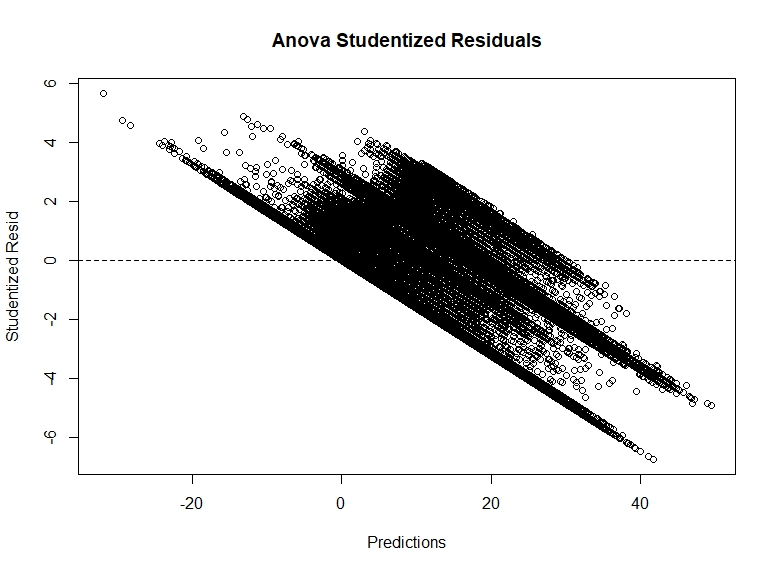
\includegraphics[width=0.9\linewidth]{img/anova/anova_studentized_residuals}
		\caption{Gráfico estandarizado de los residuos para probar la homogeneidad}
		\label{fig:anova_studentized_residuals}
	\end{figure}
	
	\begin{figure}[H]
		\centering
		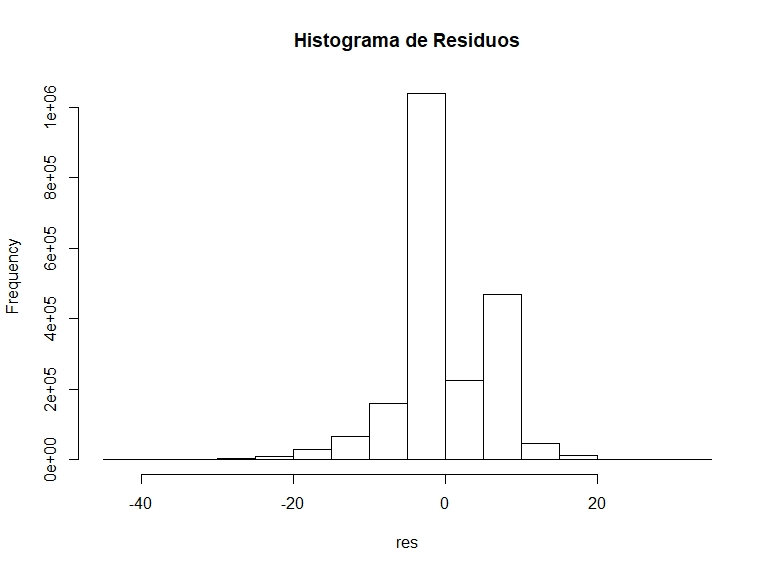
\includegraphics[width=0.9\linewidth]{img/anova/residuals_histogram}
		\caption{Histograma de los Residuos para probar normalidad}
		\label{fig:residuals_histogram}
	\end{figure}
	
	\begin{figure}[H]
		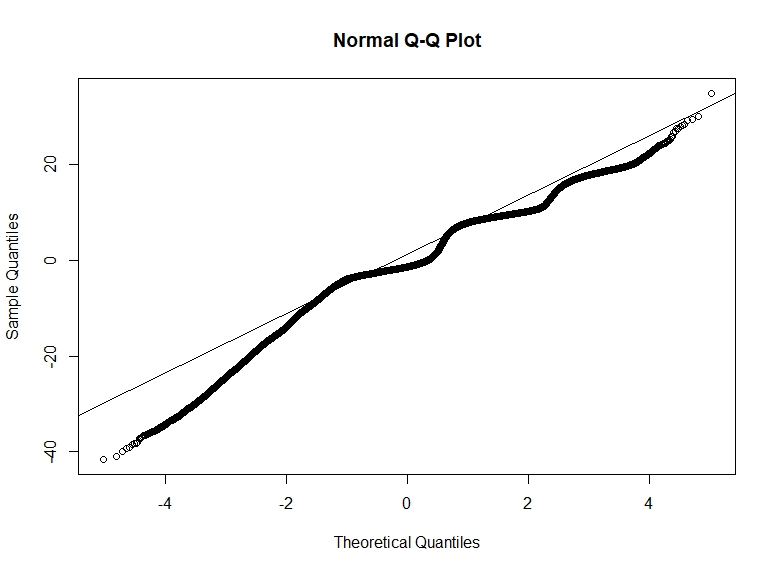
\includegraphics[width=0.9\linewidth]{img/anova/NormalQQPlot}
		\caption{Q-Q Plot para probar normalidad}
		\label{fig:NormalQQPlot}
	\end{figure}

	Como se pueden observar en el gráfico estandarizado de residuos (Figura \ref{fig:anova_studentized_residuals}), no parece tener varianza constante, el histograma de los residuos (Figura \ref{fig:residuals_histogram}) muestra un poco de comportamiento normal sin embargo, el qq-plot (Figura \ref{fig:NormalQQPlot}) presenta varias desviaciones. Parece no cumplir todos los supuestos pero probamos con los tests solo para estar seguros:
		
	\begin{figure}[H]
		\centering
		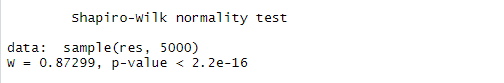
\includegraphics[width=\linewidth]{img/anova/shapiro}
		\caption{Prueba de Normalidad de Shapiro-Wilk}
		\label{fig:shapiro}
	\end{figure}

	La prueba de Shapiro-Wilk es significativa por tanto podemos rechazar $H_0$, por lo que no se cumple la hipótesis de la normalidad. Entonces, no tiene validez el experimento. Sin embargo, continuaremos con la validación de los supuestos.
	
	La prueba de Barlett no es aplicable para el análisis de la homogeneidad de las varianzas, pues se necesita que existan replicas para aplicarla. Pero por el gráfico de la Figura \ref{fig:anova_studentized_residuals} no parece que la varianza sea constante.
	 
	Por último, veamos que sucede con el test de independencia.
	
	\begin{figure}[H]
		\centering
		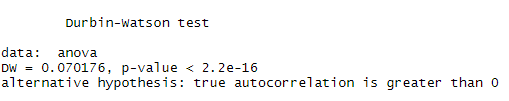
\includegraphics[width=\linewidth]{img/anova/durbin}
		\caption{Prueba de Independencia de Durbin-Watson}
		\label{fig:durbin}
	\end{figure}
	
	Se tiene que $p-valor < 0.05$ por lo que se rechaza $H_0$, lo que significa que las variables no son independientes, entonces el supuesto de independencia no se cumple tampoco.
	
	
	
%===================================================================================



%===================================================================================
% Conclusiones
% %-----------------------------------------------------------------------------------
% \section{Conclusiones}\label{sec:conc}

%   En esta sección puede incluir las conclusiones de su investigación y las ideas
%   sobre la continuidad del trabajo, en el caso que aplique.

%===================================================================================

\newpage
\newpage

%-----------------------------------------------------------------------------------
%-----------------------------------------------------------------------------------

%===================================================================================
% Bibliografía
%-----------------------------------------------------------------------------------

%-----------------------------------------------------------------------------------

\label{end}

\end{document}

%===================================================================================
